\section{Market Regimes}

Cryptocurrency markets are subject to constant change, which is reflected not only in price movements but also in the underlying structures and dynamics.
In quantitative analysis and algorithmic trading, understanding these changes is essential for developing and adapting robust trading strategies.
A central concept in this context is market regimes.

\subsection{Introduction to Market Regimes}

Market regimes describe phases with distinct statistical and economic characteristics, such as volatility, and trend behavior.
They can be understood as different "states" of the market in which certain trading patterns dominate.
Distinguishing between, for example, upward, sideways, and downward trends or high, and low volatility enables more targeted strategy selection and adaption.
Accordingly, the identification and classification of market regimes plays an increasingly important role in modern trading analysis.
For example, a strategy that performs well in a stable uptrend may fail in a sideways movement or in periods of high volatility \cite{macrosynergy-market-regime-introduction}.

Understanding market regimes leverages traders and analysts to design strategies that are adaptive, and therefore more robust.
Through targeted adaptation of the parameters or the selection of different models, the performance can be increased, and the risk can be reduced.

\subsection{How to Categorize the Market?}
\label{chap:market-regime-categories}

Categorizing different market characteristics is a common step in identifying market regimes.
In literature and practical applications, there exist different approaches to classifying markets.
A fundamental categorization is often made by the following dimensions:

\begin{enumerate}
    \item \textbf{Trend behavior:} Markets can be categorized trend following (bullish/ bearish) or trendless (sideways).
    \item \textbf{Volatility:} The volatility of a market is often an indicator for insecurity or stability.
    High volatility can indicate periods of stress, while low volatility indicates calm markets.
    \item \textbf{Liquidity:} In illiquid markets, pricing processes can be different compared to liquid markets which has effect on strategies.
\end{enumerate}

\noindent
According to the analysis goal, the categorization can be binary (e.g. bullish vs. bearish) or granular (e.g. a combination of trend behavior, and volatility).
Also, a combination of multiple indicators, named regime scores, is possible to capture more complex market structures.

In the current context, the market is categorized by trend behavior, and volatility.
This results in six categories:

\begin{enumerate}
    \item Downtrend + Low Volatility
    \item Downtrend + High Volatility
    \item Sideways Trend + Low Volatility
    \item Sideways Trend + High Volatility
    \item Uptrend + Low Volatility
    \item Uptrend + High Volatility
\end{enumerate}

\noindent
This takes into account the two most central aspects that lead traders to different trading decisions.
However, the market is not divided into too many small segments, which can lead to overfitting.

\subsection{Recognizing Market Regimes}

As described in \autoref{chap:market-regime-categories}, the market will be divided into six categories which are the result of combinations of two individual categories.
This makes it possible to categorize the two individual categories individually, and finally merge them.

\subsubsection{Recognizing Trend Behavior}
\label{chap:recognizing-trend}

The first step is to categorize the market into uptrends, downtrends, and sideways trends.
Commonly, a combination of a short-term simple moving average (e.g. SMA(50)), and a long-term simple moving average (e.g. SMA(200)) is used to identify superior trends.
The SMA(200) is considered the classic boundary between bullish and bearish market phases.
If the short-term simple moving average is above the long-term simple moving average, the market is considered bullish.
Vice versa, if the short-term simple moving average is below the long-term simple moving average, the market is considered bearish \cite{ig-regimes-mas}.

For the purpose of the current context, a modified combination of SMA(50), and SMA(100) was chosen.
This decision is based on two considerations:

\begin{enumerate}
    \item \textbf{Faster reaction:} The SMA(100) is intended to achieve faster reaction to medium-term trend changes without heavily weighting short-term volatility.
    \item \textbf{Inertia of trend definition:} A shorter trend window, compared to the SMA(200) reduces the inertia of trend definition, which can be particularly advantageous for more refined classification into uptrends, downtrends, and sideways trend.
\end{enumerate}

\noindent
Additionally, a minimum slope threshold over the last 15 minutes was integrated for the SMA(50) to avoid that minimal direction changes are mistakenly interpreted as a meaningful trend.
This short time span ensures that current market movements are adequately incorporated into the trend classification without being dominated by short-term noise (e.g., individual volatility peaks), and therefore increases the robustness of the trend recognition, and addresses the weaknesses of simple moving averages in sideways phases.
A slope above +0.05 signals a significant short-term uptrend, while a slope below -0.05 suggests a clear downtrend.
Values in between are interpreted as ambiguous, and are included in the sideways classification accordingly.

The market can therefore be divided into three trend phases based on the following criteria:

\begin{enumerate}
    \item \textbf{Uptrend:} The SMA(50) is above the SMA(100), and the slope of the SMA(50) in the last 15 minutes is greater than 0.05.
    \item \textbf{Downtrend:} The SMA(50) is below the SMA(100), and the slope of the SMA(50) in the last 15 minutes is less than -0.05.
    \item \textbf{Sideways trend:} The market currently does not meet condition 1 or 2.
\end{enumerate}

\noindent
\autoref{fig:mr-trend-classification} shows an example of trend classification of \ethusdc for 700 minutes.

\begin{figure}[H]
    \centering
    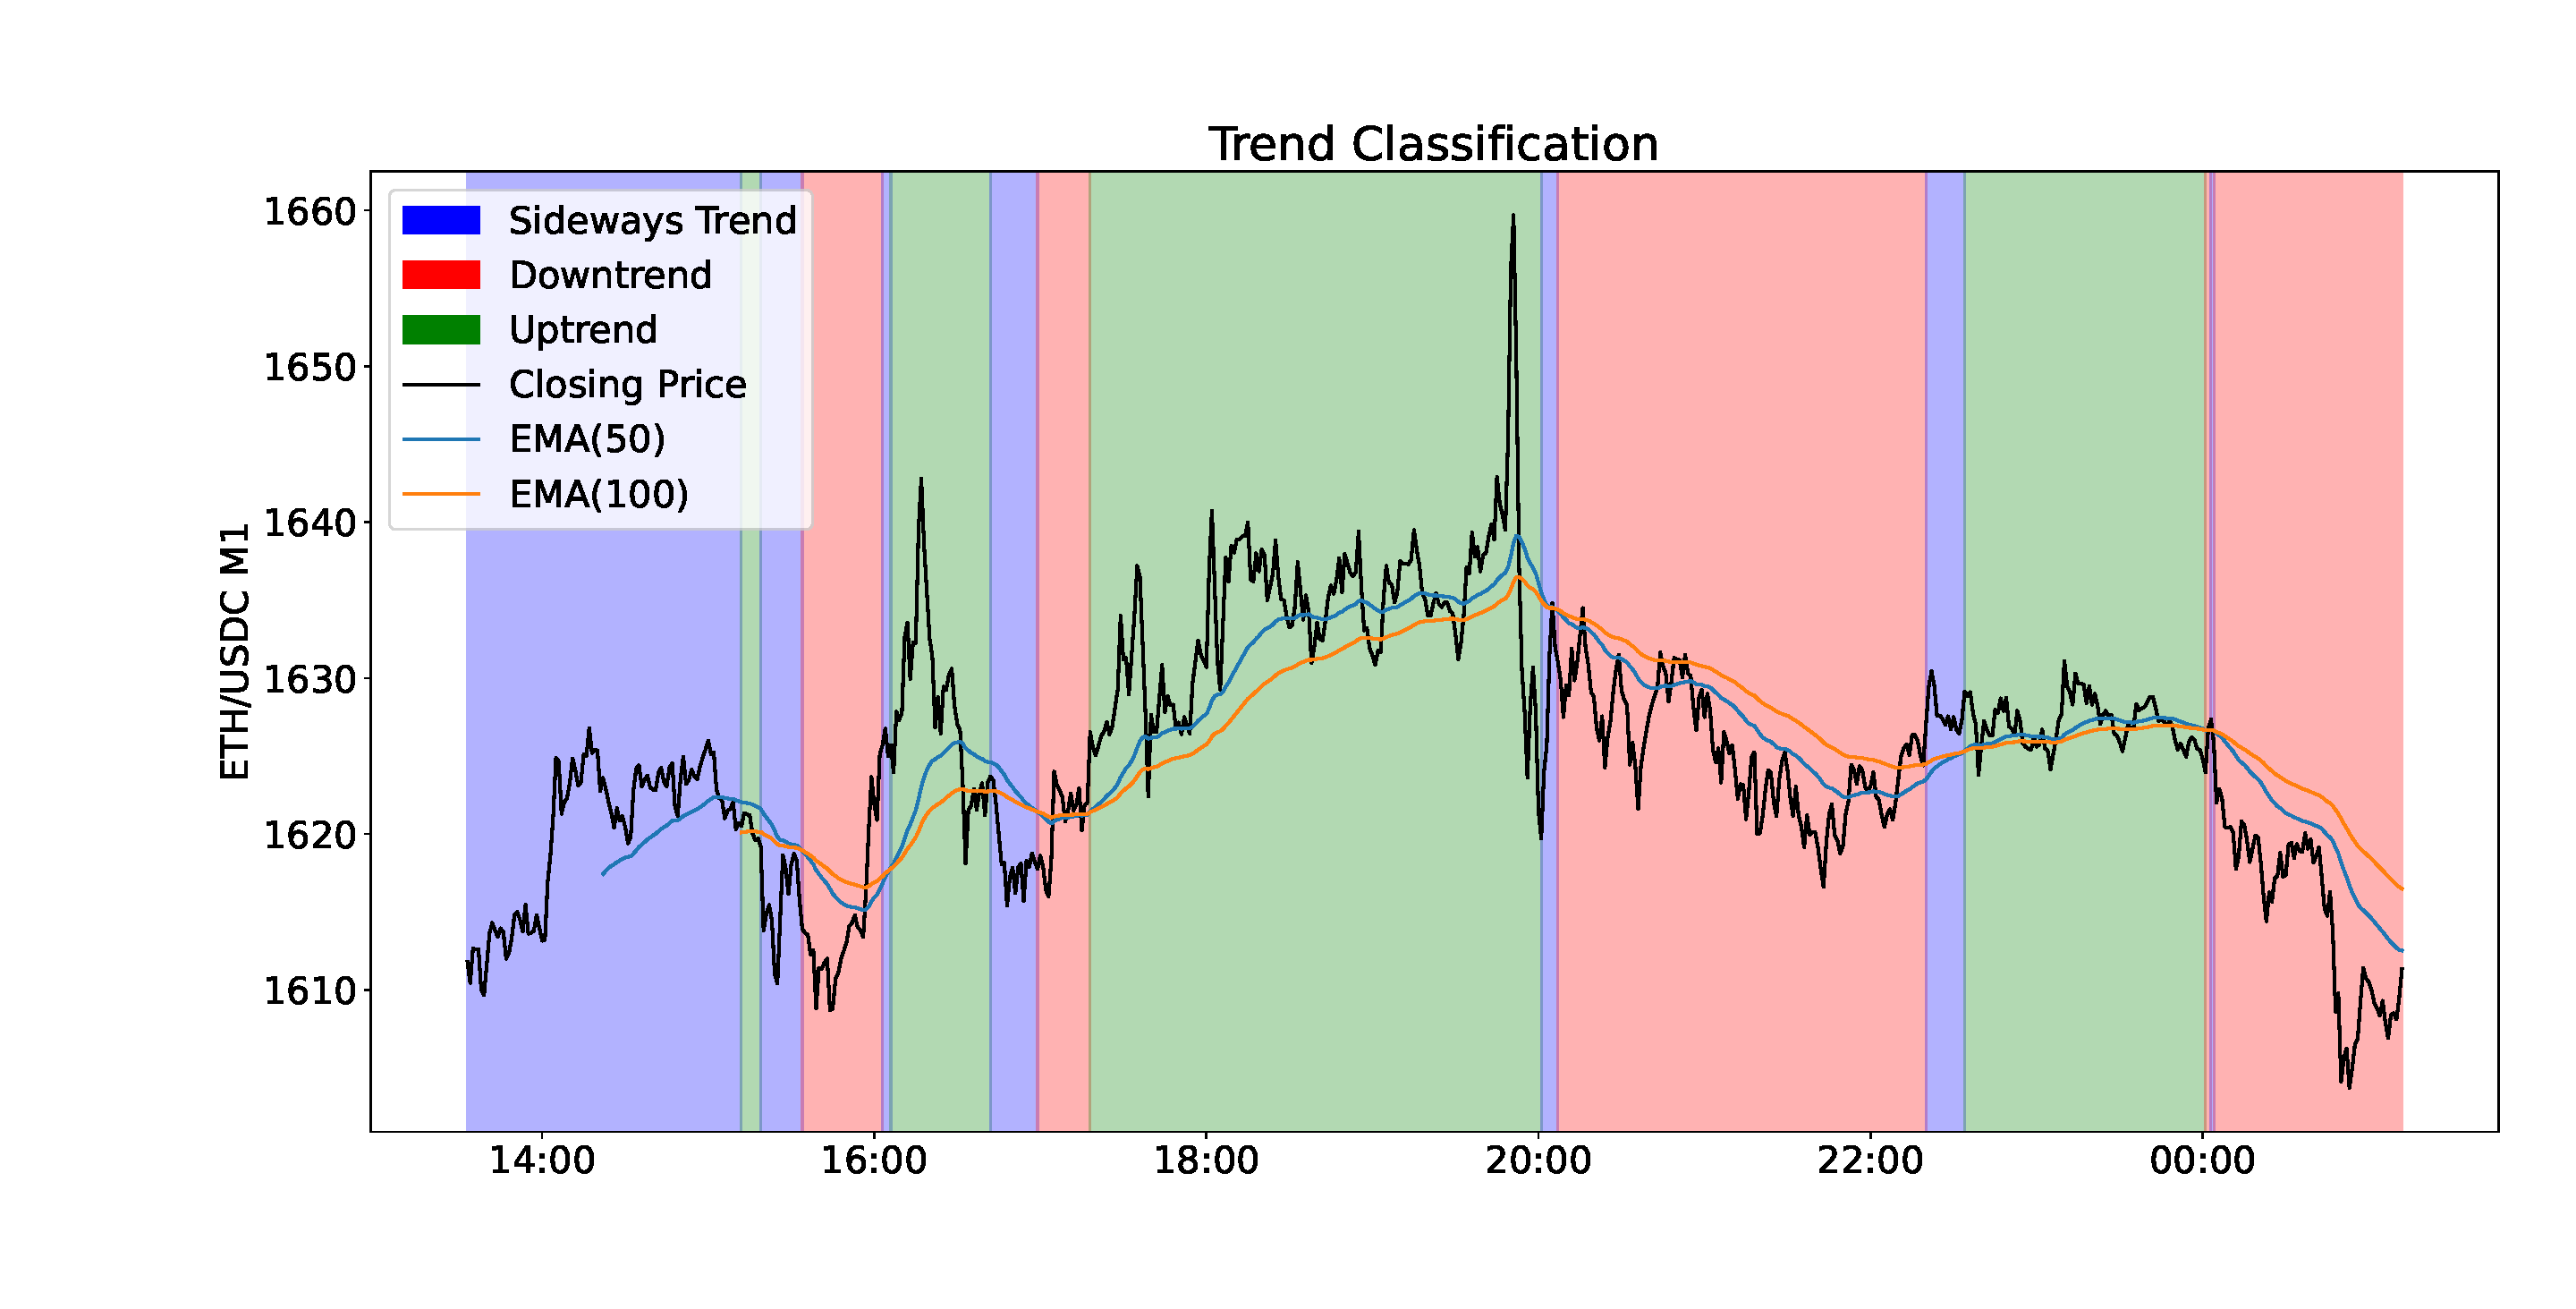
\includegraphics[width=\textwidth]{images/market-regime/market_regime_trend}
    \caption{Trend Classification}
    \label{fig:mr-trend-classification}
\end{figure}

\subsubsection{Recognizing Volatility}
\label{chap:recognizing-vola}

The second step is to categorize the market into phases with high and low volatility.
The volatility is calculated as the standard deviation of the logarithmic returns over the last 30 minutes \cite{wiki-vola}.
This locally calculated volatility depicts short-term fluctuation intensity, and enables a context-dependent assessment of current market behavior.

To classify this local volatility, a comparison is made with the median of all available volatilities in the training dataset which was used for fitting the volatility classification indicator.
If the current volatility is greater than the median, the market is classified as highly volatile.
Otherwise, the market is classified as low volatility.

This threshold definition is deliberately based on a dynamic, data-dependent approach rather than using a fixed absolute threshold.
This automatically adapts the volatility classification to each specific market, and can therefore theoretically be applied to other financial markets.

\autoref{fig:mr-vola-classification} shows the volatility classification on the same base data used in \autoref{fig:mr-trend-classification}.

\begin{figure}[H]
    \centering
    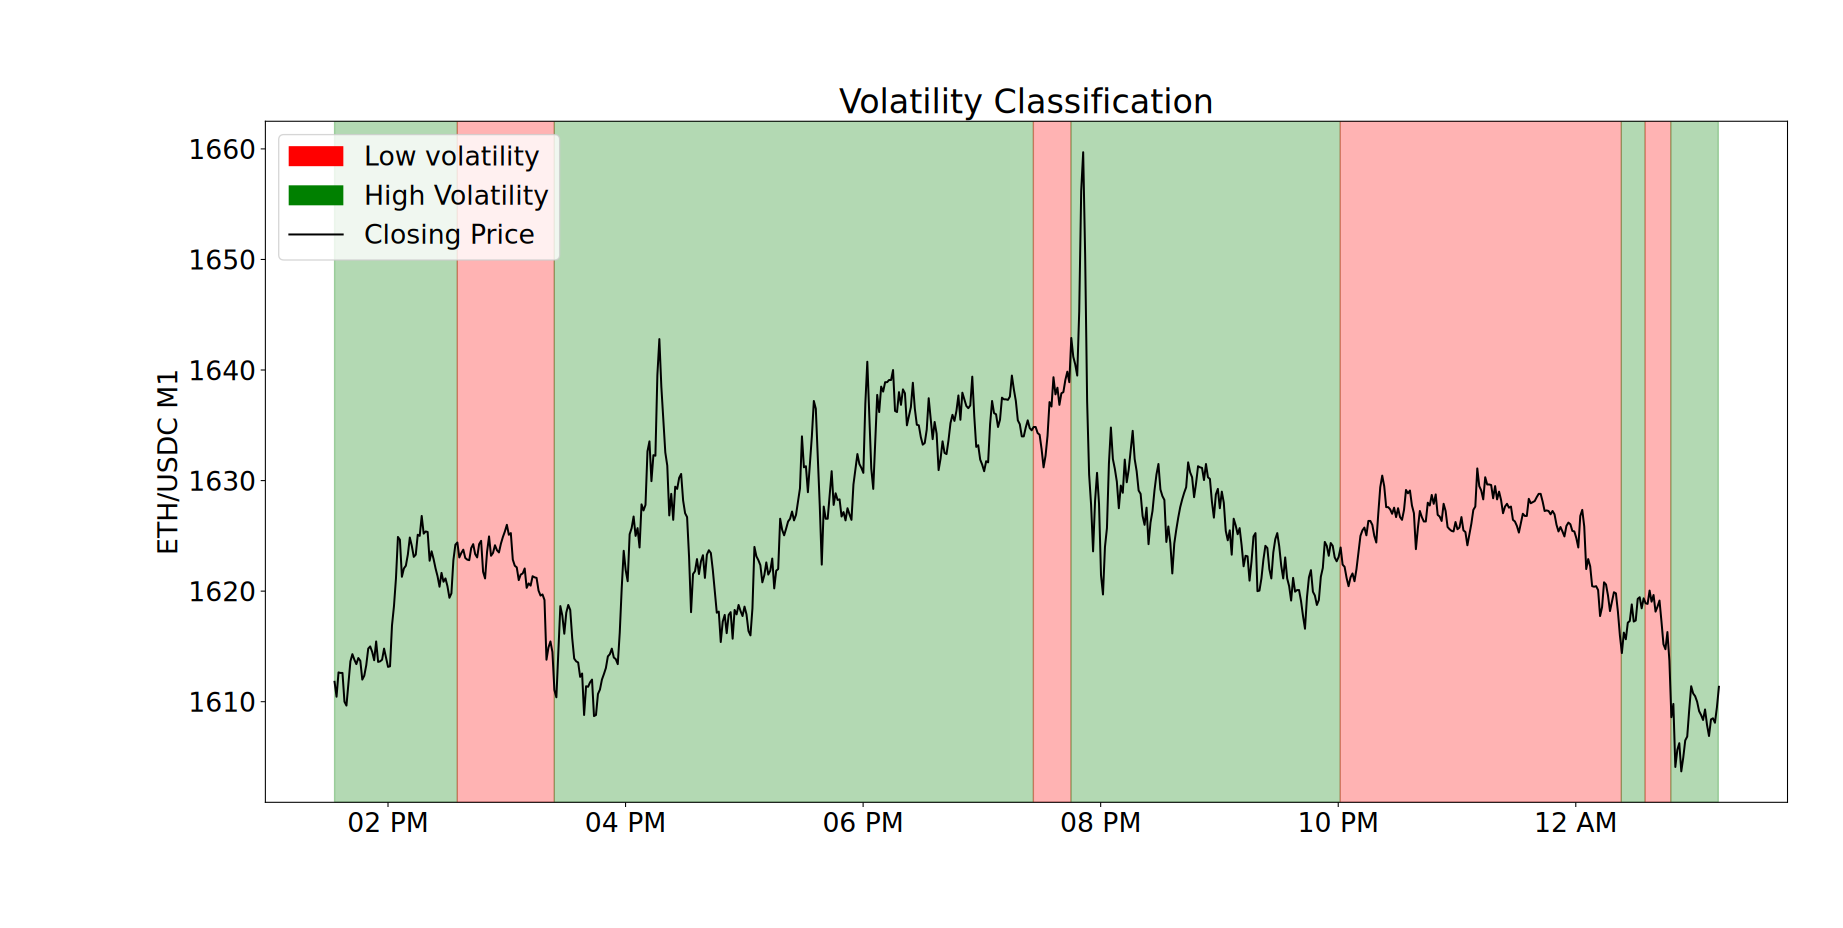
\includegraphics[width=\textwidth]{images/market-regime/market_regime_vola}
    \caption{Volatility Classification}
    \label{fig:mr-vola-classification}
\end{figure}

\subsubsection{Combining Trend and Volatility Classification}

After the two separate classifications in \autoref{chap:recognizing-trend} and \autoref{chap:recognizing-vola} the results can be combined.
The results of the combination can be seen in \autoref{fig:mr-classification}.

\begin{figure}[H]
    \centering
    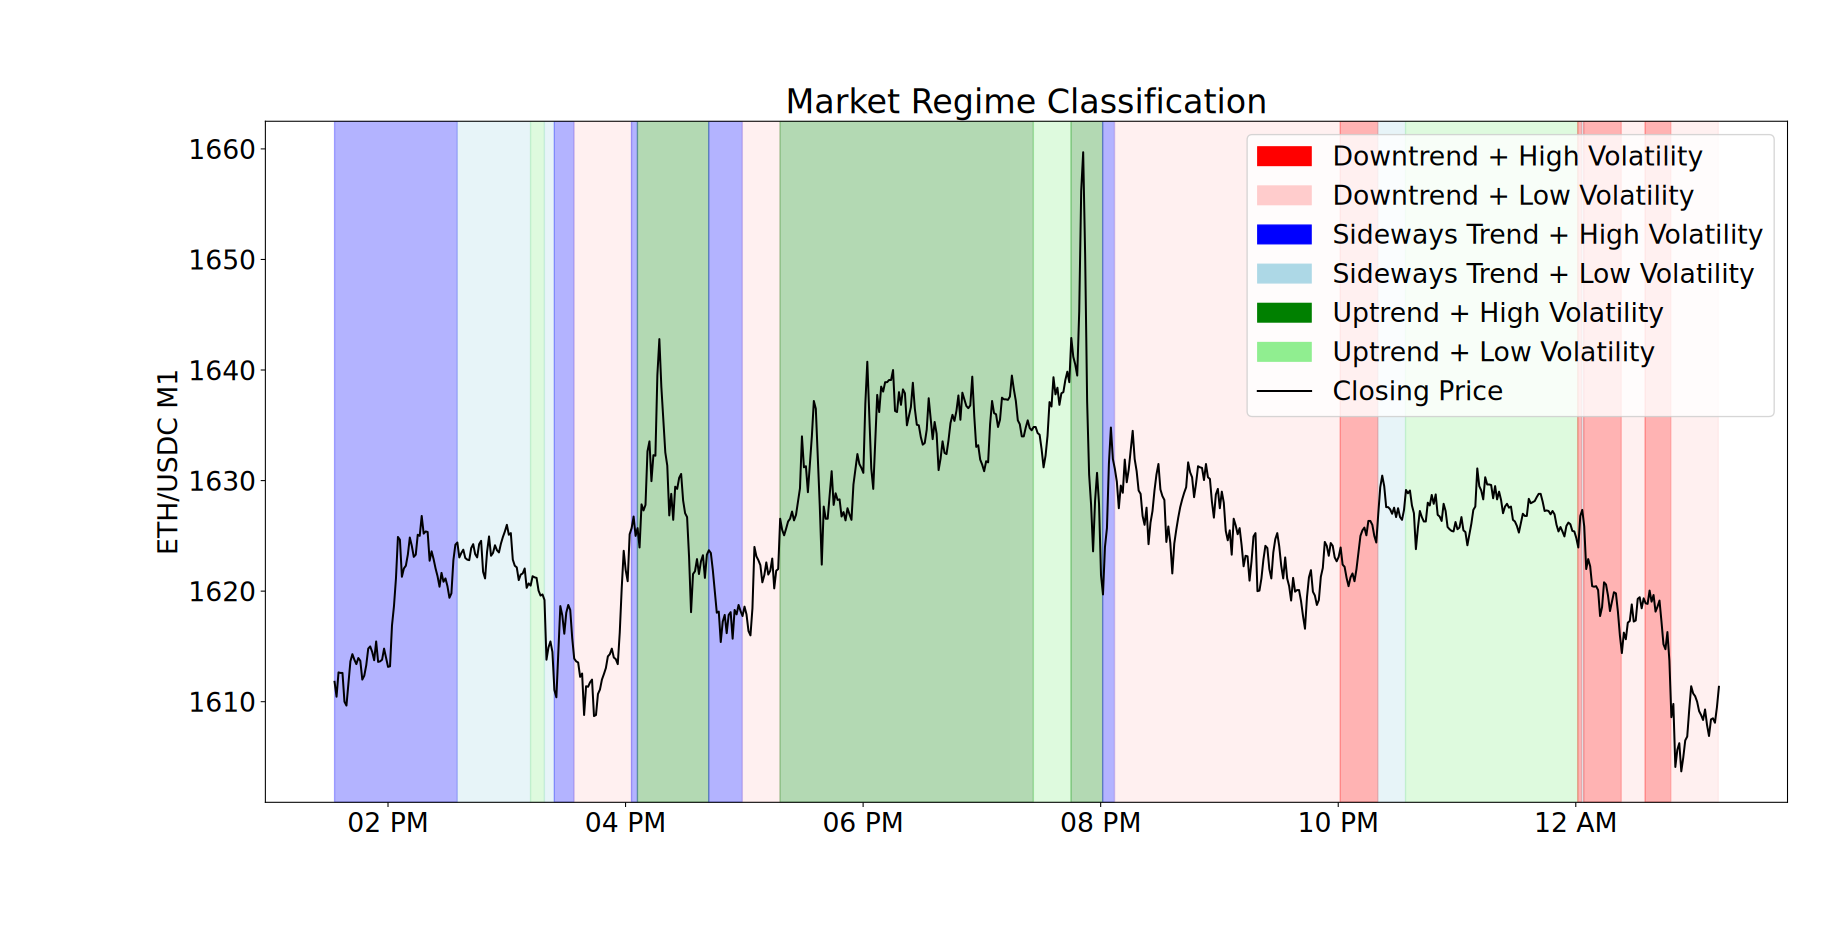
\includegraphics[width=\textwidth]{images/market-regime/market_regime}
    \caption{Regime Classification}
    \label{fig:mr-classification}
\end{figure}

\noindent
While classification of the market regimes some discrepancies may occur in individual cases between the algorithmically determined category and the visually perceived category.
Such misclassifications are particularly possible during transition phases or in the case of short-term outliers.
For example, the downtrend, highly volatile market regime after 10:00 PM, the algorithm detected a downtrend, but visually, an uptrend is perceived.
At this time, the market is in a transition, which causes this misclassification.

Crucially, the classification distinguishes consistently and meaningfully, which is the case when viewed as a whole.
The robustness and usefulness of the approach does not arise from absolute freedom from errors, but rather from the systematic reduction of uncertainty compared to a purely visual or subjective assessment.

\subsection{Dividing Market Regimes in Durations}

Based on the combination of trend direction and volatility level, the duration of each market regime is also taken into account to enable a more differentiated classification.
The regime duration is divided into three quantiles (33\%, 66\%, 100\%) based on its distribution, allowing for classification into short-term, medium-term, and long-term phases.
The notation in the current work for the respective regime durations is $Q_{0.33}$, $Q_{0.66}$ and $Q_{1}$.

The combination of these three dimensions results in a total of 18 different market regimes.
This fine-grained segmentation makes it possible to more precisely capture and differentiate different market conditions.
For example, a short-term, volatile uptrend from a long-term, calm downtrend.

Even through this makes the market appear more fragmented, and regimes can change more frequently, this finer subdivision is analytically useful.
It allows for context-sensitive market behavior to be examined, and differences in the dynamics of effectiveness of trading strategies in specific regime types to be systematically analyzed.

Instead of smoothing out reality with overly broad categories, a more nuanced picture is deliberately drawn that takes into account both the direction, intensity, and stability of market behavior.
The resulting increased complexity is not a disadvantage, but rather a prerequisite for more meaningful, context-based analyses.

